\documentclass[11pt]{article}
\usepackage[letterpaper,margin=1in]{geometry}
\usepackage[T1]{fontenc}
\usepackage{lmodern}
\usepackage{amsmath,amssymb,bm}
\usepackage{graphicx}
\usepackage{xcolor}
\usepackage[hidelinks]{hyperref}
\usepackage{caption}
\usepackage[section]{placeins}
\captionsetup{font=small,labelfont=bf}
\definecolor{acc}{HTML}{2A78D6}
\newcommand{\dev}{\operatorname{dev}}
\newcommand{\nb}[1]{\texttt{#1}}
\title{Differentiable plasticity FEM in JAX\\[4pt]\large what a mechanical test sees, and how its derivatives flow}
\author{Raj Mahat\\ \small Georgia Institute of Technology}
\date{Learning notes, October 2026}
\begin{document}
\maketitle

\noindent These notes build a small, fully differentiable finite-element model of a punch test on an
elastic--plastic plate, and use it to follow how a change in the hardening law travels through the
computation to the measured load. The model was written on core JAX; the figures come from it or are
drawn in TikZ.
The material, geometry and parameter values are generic and chosen for teaching.

\tableofcontents

%=====================================================================
\section{What a mechanical test sees}
%=====================================================================
A test imposes boundary data (a displacement, a traction, contact with a fixture) and a loading path.
The body responds with fields $u(x,t)$, $\varepsilon(x,t)$, $\sigma(x,t)$ and internal variables
$q(x,t)$. We observe only a compressed record: here the punch load at each depth,
$y = \{L(d_k)\}_{k=1}^{N_d}$. The constitutive law is never measured directly. It reaches the data only
after passing through the local plastic response, equilibrium with contact, the loading history and the
readout (Fig.~\ref{fig:chain}). Calibration is therefore an inverse problem,
\begin{equation}
  y_{\rm obs} = \mathcal G(\theta) + \epsilon ,
\end{equation}
and the derivative $\partial\mathcal G/\partial\theta$ is the object that tells us what the test can say
about $\theta$.

\begin{figure}[h]\centering
\includegraphics[width=\linewidth]{figs/tikz/fc3_chain.pdf}
\caption{The chain from the hardening law to the measured load.}\label{fig:chain}
\end{figure}

%=====================================================================
\section{J\textsubscript{2} plasticity with combined hardening}
%=====================================================================
With $s=\dev\sigma$, back stress $X$ and accumulated plastic strain $p$,
\begin{align}
  f &= \sigma_{eq}(s - X) - \sigma_y(p) \le 0, &
  \sigma_{eq}(\xi) &= \sqrt{\tfrac32\,\xi:\xi},\\
  \dot\varepsilon^p &= \dot\gamma\, n, \quad n = \tfrac32\,\frac{\xi}{\sigma_{eq}(\xi)}, &
  \dot p &= \dot\gamma,\\
  \sigma_y(p) &= \sigma_0 + Q\,(1-e^{-\beta p}) &&\text{(Voce, isotropic)},\\
  \dot X &= \tfrac23 C\,\dot\varepsilon^p - \gamma_k\,\dot p\,X &&\text{(Armstrong--Frederick, kinematic)}.
\end{align}
Isotropic hardening grows the elastic domain; kinematic hardening moves it (Fig.~\ref{fig:yield}).
Under a load reversal the second gives early reverse yielding, the Bauschinger effect
(Fig.~\ref{fig:uniaxial}). Positivity of $\sigma_y(0)$ and $\sigma_y'\ge 0$ keep the incremental
problem well posed. In tabulated form (as in commercial codes) $\sigma_y$ is simply a function of $p$;
here we use the three-parameter Voce chart $\theta=(\sigma_0,Q,\beta)$.

\begin{figure}[h]\centering
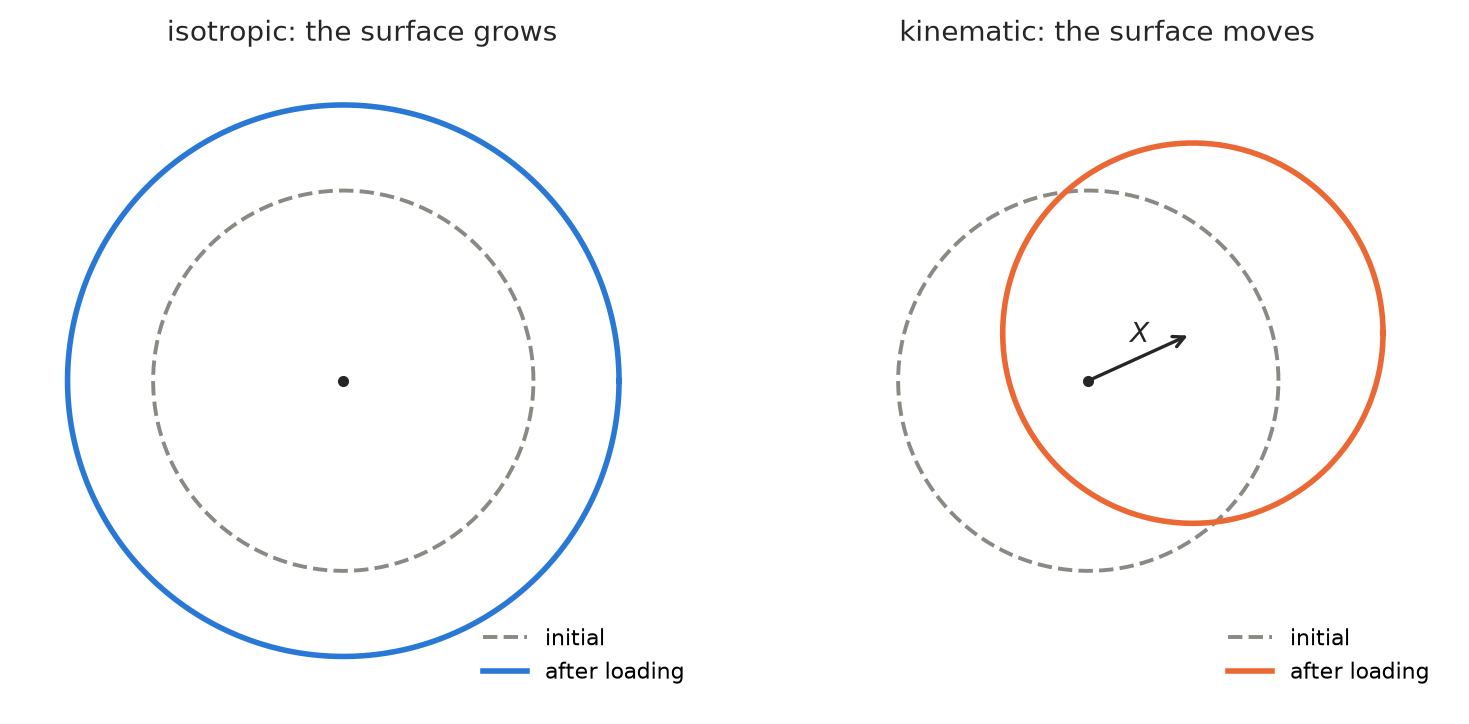
\includegraphics[width=0.78\linewidth]{figs/yield_surfaces.png}
\caption{Deviatoric-plane view: isotropic hardening dilates the surface, kinematic hardening translates it by $X$.}\label{fig:yield}
\end{figure}
\begin{figure}[h]\centering
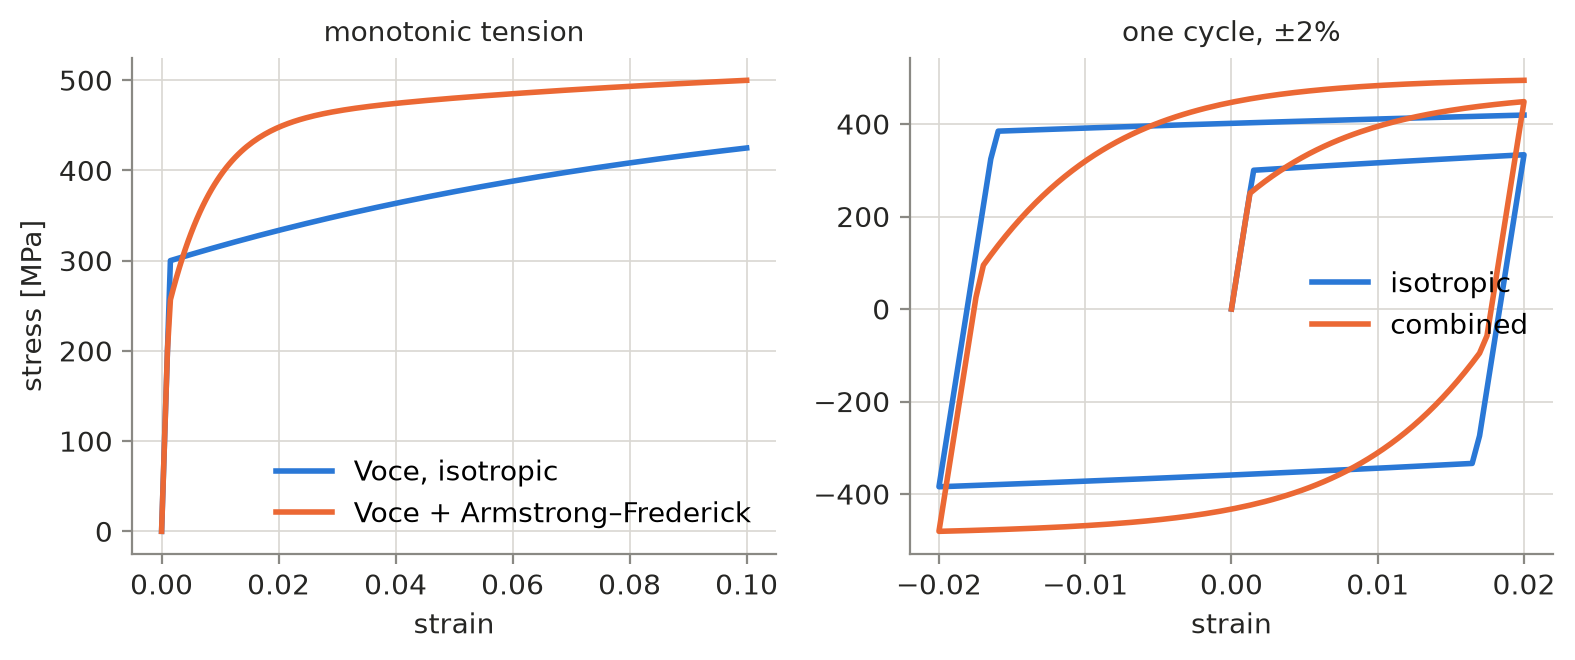
\includegraphics[width=0.85\linewidth]{figs/uniaxial_curves.png}
\caption{Monotonic tension and one strain cycle for pure Voce and for Voce + Armstrong--Frederick.}\label{fig:uniaxial}
\end{figure}

%=====================================================================
\section{The return map and its Jacobian}
%=====================================================================
Backward Euler over an increment, with local unknowns $v=(\sigma,\varepsilon^p,X,p)$, gives the local
residual $h(v)=0$ (Fig.~\ref{fig:local}): elastic update, flow rule, back-stress evolution, accumulation
and yield consistency. Starting from the trial state $s^{\rm tr}=2G\,\dev(\varepsilon-\varepsilon^p_{n})$,
everything collapses to one scalar equation for $\Delta\gamma$:
\begin{equation}
  g(\Delta\gamma) = \Big\| s^{\rm tr} - \frac{X_n}{1+\gamma_k\Delta\gamma}\Big\|
  - \Big(2G\sqrt{\tfrac32} + \sqrt{\tfrac23}\,\frac{C}{1+\gamma_k\Delta\gamma}\Big)\Delta\gamma
  - \sqrt{\tfrac23}\,\sigma_y(p_n+\Delta\gamma) = 0 .
\end{equation}
In code this root is found with Newton inside \nb{jax.lax.custom\_root}. The implicit function theorem then
gives every derivative of the result without differentiating through the iterations:
\begin{equation}
  \frac{d\Delta\gamma}{d(\cdot)} = -\Big(\frac{\partial g}{\partial\Delta\gamma}\Big)^{-1}\frac{\partial g}{\partial(\cdot)} .
\end{equation}
The algorithmic (consistent) tangent $\mathbb D=\partial\sigma_{n+1}/\partial\varepsilon_{n+1}$ is then a
single \nb{jax.jacfwd}. For pure isotropic hardening it agrees with the textbook closed form
\begin{equation}
  \mathbb D = K\,\mathbf 1\otimes\mathbf 1 + 2G\theta_1\,\mathbb I_{\rm dev} - 2G\theta_2\,\hat n\otimes\hat n,\qquad
  \theta_1 = 1-\frac{3G\Delta\gamma}{\sigma_{eq}^{\rm tr}},\quad
  \theta_2 = \frac{1}{1+H/3G}-(1-\theta_1),
\end{equation}
to round-off, and it needs no change for the combined model.

\begin{figure}[h]\centering
\includegraphics[width=0.82\linewidth]{figs/tikz/fc5_local.pdf}
\caption{The local residual and the map from a local stress change to nodal force.}\label{fig:local}
\end{figure}

%=====================================================================
\section{The incremental finite-element problem}
%=====================================================================
Per increment three residuals are coupled (Fig.~\ref{fig:forward}): the local constitutive residual
$h_k$ at every Gauss point, global equilibrium $r_k$, and the contact conditions. Newton solves the
linearized saddle problem; condensing the local solve into the global one gives the consistent tangent
\begin{equation}
  K_k = r_U - r_v\,h_v^{-1}\,h_U ,
\end{equation}
the material's response to nodal motion. Because $K_k$ is exact, Newton converges quadratically once
the contact set settles.

The teaching model is an axisymmetric clamped plate (radius 2\,mm, thickness 0.5\,mm) pressed by a rigid
ball (radius 1.25\,mm). It uses 4-node quads with $2\times2$ Gauss points, small strain, and frictionless
penalty contact, so the saddle reduces to $K_k\,\delta U = -r_k$ with the penalty stiffness inside $K_k$.
The pieces map one-to-one onto JAX (Fig.~\ref{fig:jax}): the internal force is the transpose of the
strain map (\nb{jax.vjp}), the tangent is \nb{jax.jacfwd} of the residual, and the global Newton also sits
in \nb{custom\_root}, so $\partial U/\partial(\cdot) = -K^{-1}\partial R/\partial(\cdot)$ is applied
directly.

\begin{figure}[p]\centering
\includegraphics[width=\linewidth]{figs/tikz/fc1_forward.pdf}
\caption{The forward solve for one increment, with the residuals it balances and the condensed tangent.}\label{fig:forward}
\end{figure}
\begin{figure}[h]\centering
\includegraphics[width=\linewidth]{figs/tikz/fc6_solve_readout.pdf}
\caption{Kinematics, the constrained solve, the state update and the readout.}\label{fig:prims}
\end{figure}
\begin{figure}[h]\centering
\includegraphics[width=0.62\linewidth]{figs/tikz/fc4_jax.pdf}
\caption{Which JAX tool does which job.}\label{fig:jax}
\end{figure}
\begin{figure}[h]\centering
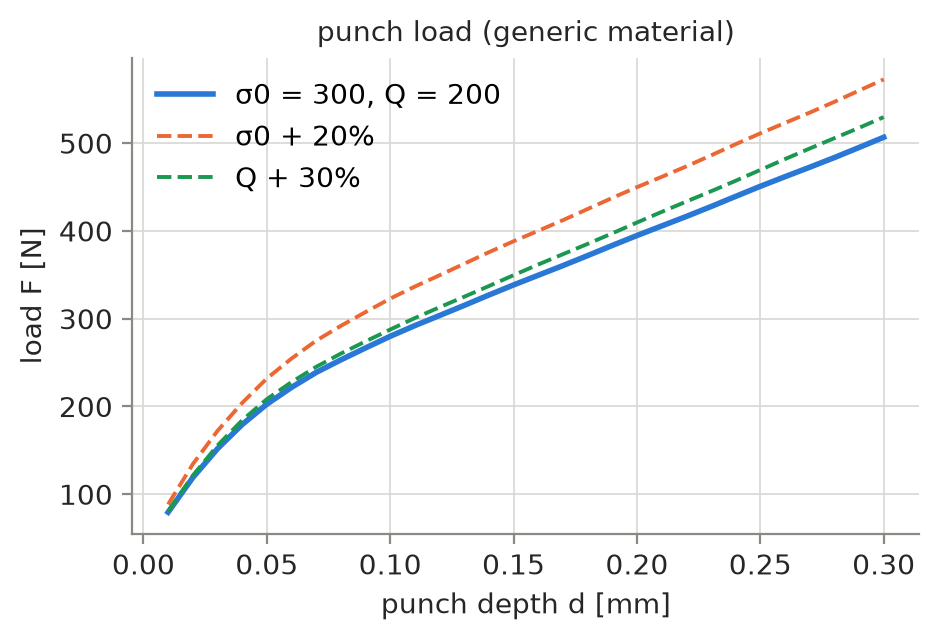
\includegraphics[width=0.49\linewidth]{figs/punch_load.png}\hfill
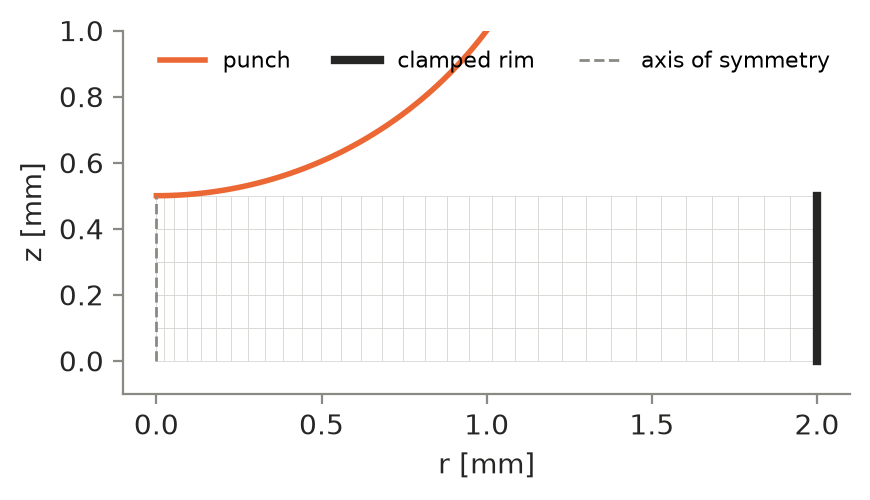
\includegraphics[width=0.49\linewidth]{figs/punch_mesh.png}\\[4pt]
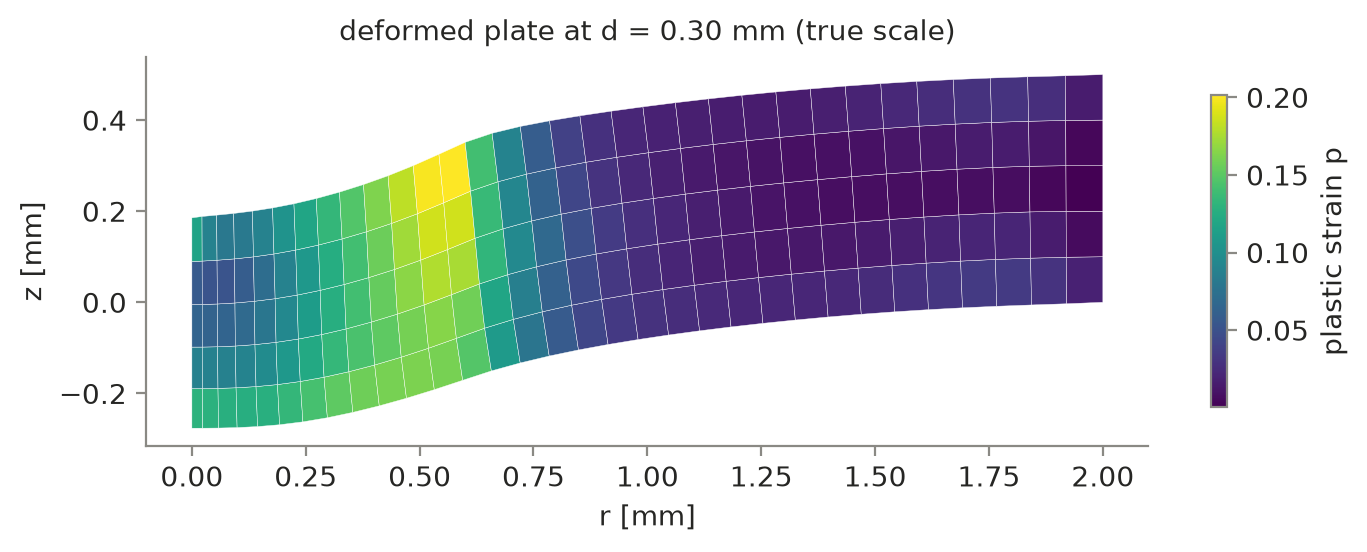
\includegraphics[width=0.8\linewidth]{figs/punch_fields.png}
\caption{Load--depth curves (with two parameter changes), the mesh, and accumulated plastic strain at the last increment.}\label{fig:punch}
\end{figure}

%=====================================================================
\section{Linearizing the forward model}
%=====================================================================
A parameter change enters in one place: the yield row, evaluated at the plastic strain reached at each
plastic Gauss point,
\begin{equation}
  \frac{\partial h^f}{\partial\theta}\Big|_g = -\frac{\partial\sigma_y}{\partial\theta}\big(p_k(x_g);\theta\big).
\end{equation}
From there it is \emph{resisted} by the local block $h_v^{-1}$, \emph{redistributed} by equilibrium under
contact (the same factorized $K_k$ as the forward Newton, one extra right-hand side), \emph{carried} to later
increments through the committed state, and \emph{read out} as a change in load (Fig.~\ref{fig:sens}).
With $s_k=\partial q_k/\partial\theta$, the pseudoload and the state recursion are
\begin{align}
  f_{H,k} &= r_v\,h_v^{-1}\big(h_{q_{k-1}}s_{k-1}+h_\theta\big) + f_{\Gamma,k},\\
  s_k &= -S_q\,h_v^{-1}\big(h_\varepsilon B\,U_{\theta,k} + h_{q_{k-1}}s_{k-1} + h_\theta\big).
\end{align}
Writing $s_k=\Phi_k s_{k-1}+\Upsilon_k\,\delta\theta$ and unrolling (Fig.~\ref{fig:rec}) shows that every
increment injects, and the number of carry steps on a path is how old that injection is. Assembled, the
Jacobian factors as
\begin{equation}
  J = \mathcal D + \mathcal H\circ(\mathrm{Id}-\mathcal T)^{-1}\circ\mathcal G ,
  \qquad (\mathrm{Id}-\mathcal T)^{-1} = \textstyle\sum_{n=0}^{N-1}\mathcal T^n ,
\end{equation}
a finite Neumann series because the history transfer $\mathcal T$ is strictly causal (Fig.~\ref{fig:jac}).
Inside each operator the same two paths appear, one ending in the state and one in the load
(Fig.~\ref{fig:engines}).

\paragraph{Direct or adjoint.} Direct evaluation fills $J$ column by column (one extra solve per
parameter per increment); adjoint fills it row by row (one backward sweep per output). With three
parameters and thirty depths, direct is cheaper; with many parameters and a scalar objective, adjoint is.
In JAX these are \nb{jacfwd} and \nb{jacrev}. Both were checked, together with finite differences and a
hand-written direct recursion, against each other (Fig.~\ref{fig:sensnum}).

\begin{figure}[p]\centering
\includegraphics[width=\linewidth]{figs/tikz/fc2_sensitivity.pdf}
\caption{Sensitivity rides the same structure as the forward solve.}\label{fig:sens}
\vspace{10pt}
\includegraphics[width=0.85\linewidth]{figs/tikz/fc7_recursion.pdf}
\caption{(a) The recursion for one increment. (b) Unrolled over increments, one injection highlighted.}\label{fig:rec}
\end{figure}
\begin{figure}[h]\centering
\includegraphics[width=0.72\linewidth]{figs/tikz/fc9_jacobian.pdf}
\caption{The assembled Jacobian, factor by factor.}\label{fig:jac}
\end{figure}
\begin{figure}[h]\centering
\includegraphics[width=0.92\linewidth]{figs/tikz/fc8_engines.pdf}
\caption{Inside the operators: the state path and the load path, each fed by the parameter source and the history source.}\label{fig:engines}
\end{figure}
\begin{figure}[h]\centering
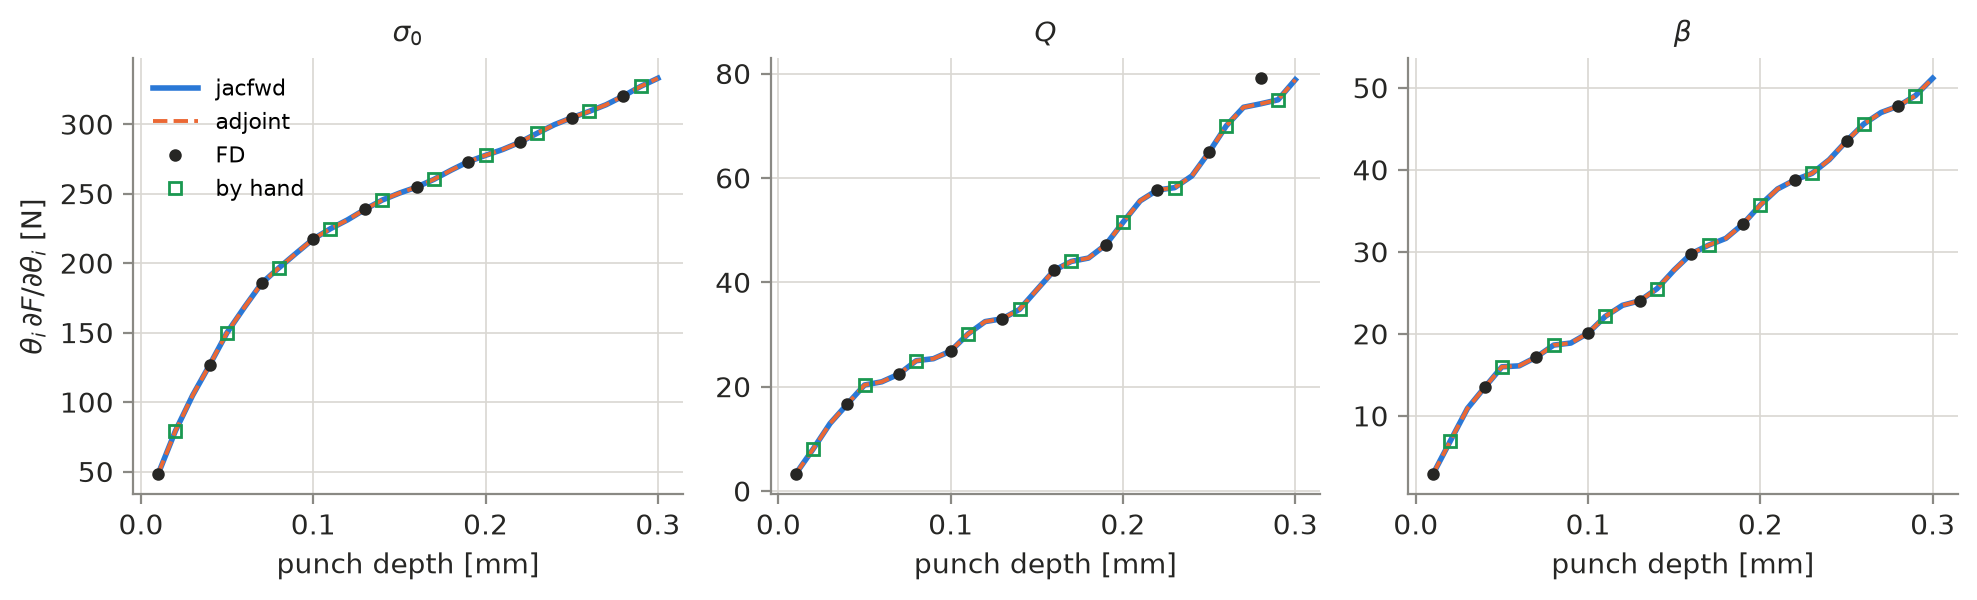
\includegraphics[width=\linewidth]{figs/punch_sensitivity.png}
\caption{$\theta_i\,\partial L/\partial\theta_i$ for the punch: forward mode, adjoint, finite differences and the hand-written recursion agree.}\label{fig:sensnum}
\end{figure}

%=====================================================================
\section{A local Bayesian view with three parameters}
%=====================================================================
Linearize at $\theta_0$: $\mathcal G(\theta_0+\delta\theta)\approx\mathcal G(\theta_0)+J\,\delta\theta$,
with noise $\epsilon\sim\mathcal N(0,\Sigma)$. Then
\begin{equation}
  \mathcal J(\theta) = \tfrac12\|y-\mathcal G(\theta)\|^2_{\Sigma^{-1}} + \tfrac12\|\theta-\theta_{\rm pr}\|^2_{Q_{\rm pr}},
  \qquad Q_{\rm post}\approx Q_{\rm pr} + \Gamma,\qquad \Gamma = J^{\top}\Sigma^{-1}J .
\end{equation}
$\Gamma$ (the Fisher information, or Gauss--Newton Hessian) carries everything the experiment
contributes locally. Its generalized eigenpairs $\Gamma\psi_i=\lambda_i\,Q_{\rm pr}\psi_i$ give the
directions the data inform: along mode $i$ the posterior variance is the prior variance times
$1/(1+\lambda_i)$, so modes with $\lambda_i>1$ have their variance at least halved. Comparing
$\Gamma$ for tension and for the punch (Fig.~\ref{fig:fisher}) shows which combinations of
$(\sigma_0,Q,\beta)$ each test pins down. All of this is local: one anchor, one noise model, one
three-parameter chart.

\begin{figure}[h]\centering
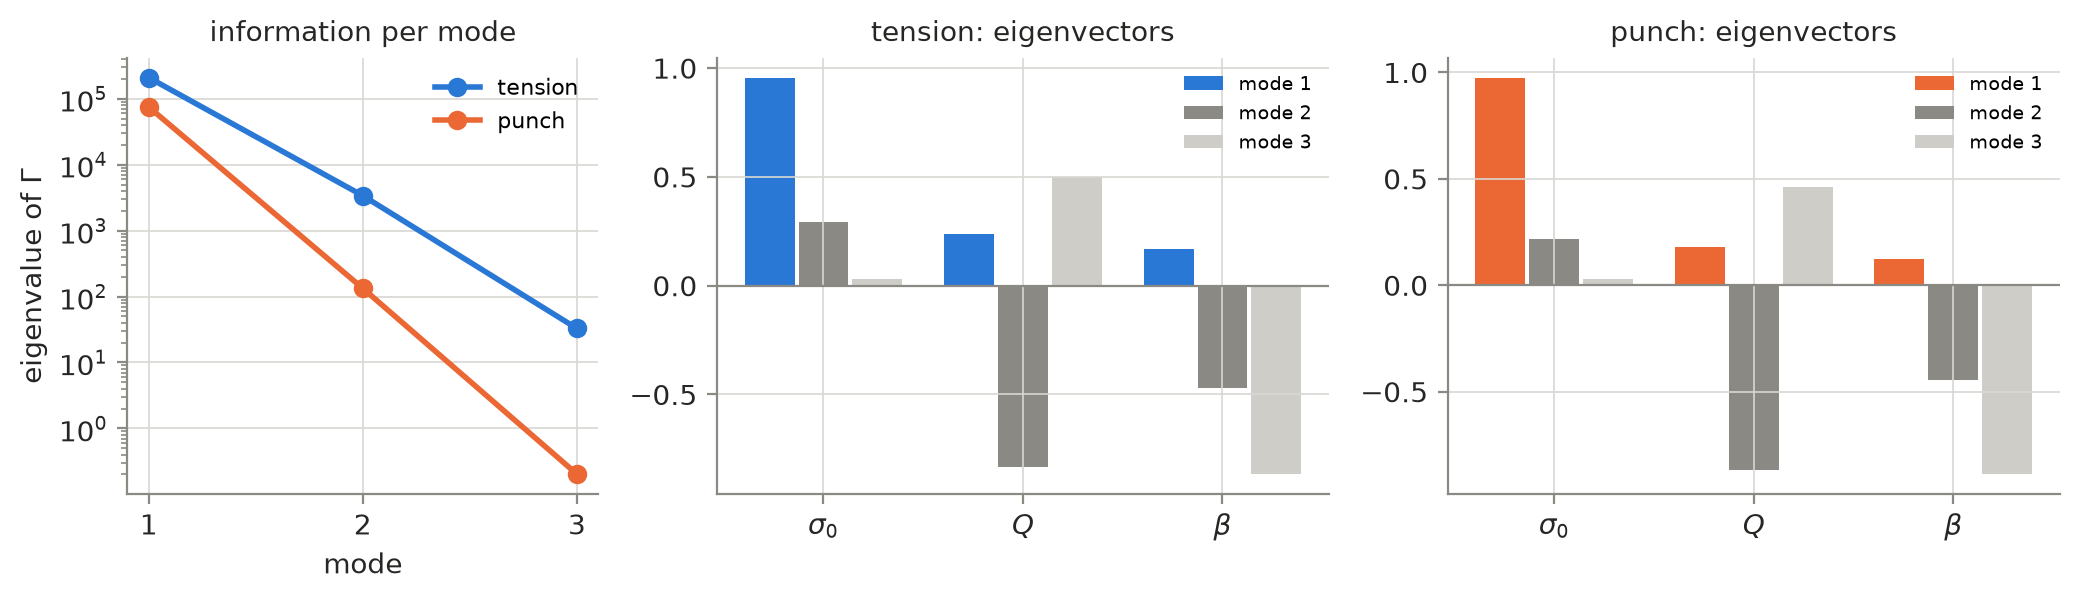
\includegraphics[width=\linewidth]{figs/fisher_modes.png}
\caption{Eigenvalues and eigenvectors of $\Gamma$ in log-parameters, 1\% noise relative to each test's peak.}\label{fig:fisher}
\end{figure}

%=====================================================================
\section{Where this leads}
%=====================================================================
The same machinery can be asked a sharper question: not ``how does the load change with three
constants'' but ``where in plastic-strain space, at each depth, is the load sensitive to the hardening
law at all''. Figure~\ref{fig:teaser} is a first look (work in progress).

\begin{figure}[h]\centering
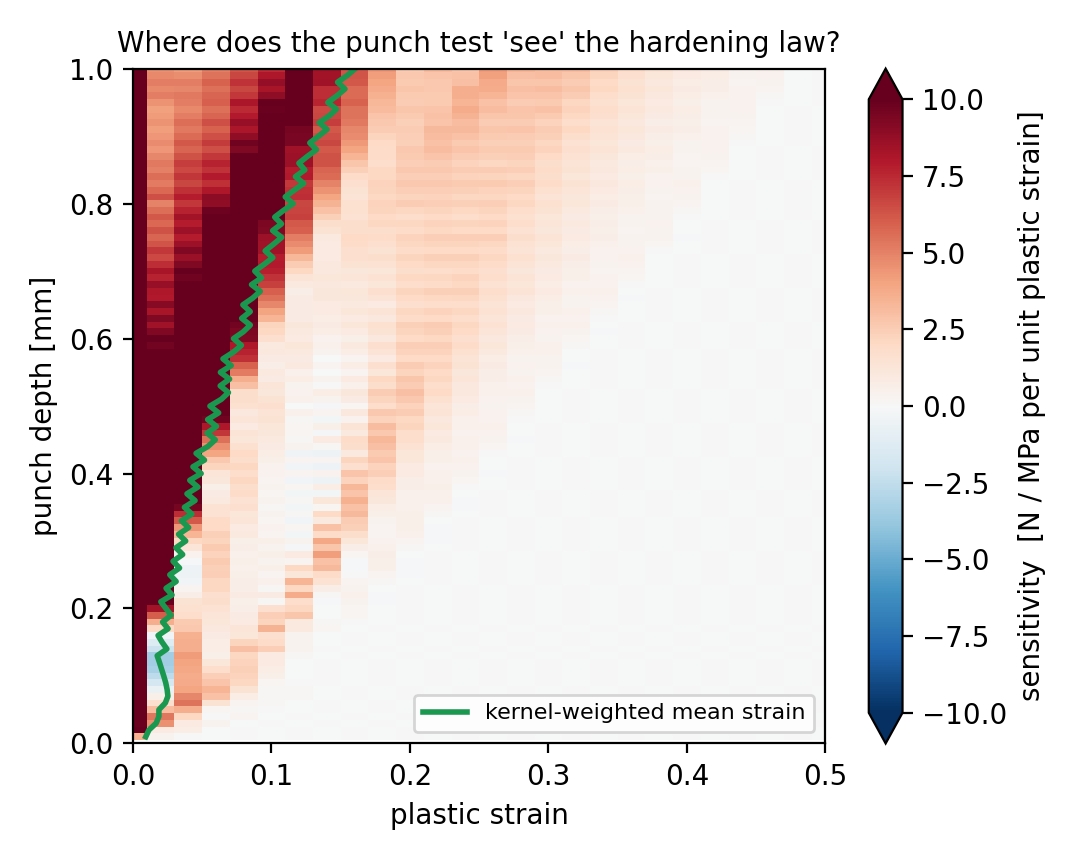
\includegraphics[width=0.62\linewidth]{figs/teaser_kernel.png}
\caption{Work in progress: sensitivity of the punch load to the hardening law, resolved in plastic strain, with the kernel-weighted mean strain.}\label{fig:teaser}
\end{figure}

\section*{References}
\begin{itemize}\small
\item J.\,C.\ Simo and T.\,J.\,R.\ Hughes, \emph{Computational Inelasticity}, Springer (1998).
\item E.\,A.\ de Souza Neto, D.\ Peri\'c and D.\,R.\,J.\ Owen, \emph{Computational Methods for Plasticity}, Wiley (2008).
\item J.-L.\ Chaboche, A review of some plasticity and viscoplasticity constitutive theories, \emph{Int.\ J.\ Plasticity} 24 (2008) 1642--1693.
\item P.\,J.\ Armstrong and C.\,O.\ Frederick, A mathematical representation of the multiaxial Bauschinger effect (1966); reprinted in \emph{Materials at High Temperatures} 24 (2007) 1--26.
\item P.\ Wriggers, \emph{Computational Contact Mechanics}, 2nd ed., Springer (2006).
\item M.\ Kleiber, H.\ Ant\'unez, T.\,D.\ Hien and P.\ Kowalczyk, \emph{Parameter Sensitivity in Nonlinear Mechanics}, Wiley (1997).
\item P.\ Michaleris, D.\,A.\ Tortorelli and C.\,A.\ Vidal, Tangent operators and design sensitivity formulations for transient non-linear coupled problems, \emph{Int.\ J.\ Numer.\ Meth.\ Eng.} 37 (1994) 2471--2499.
\item M.\ Blondel et al., Efficient and modular implicit differentiation, \emph{NeurIPS} (2022).
\item J.\ Bradbury et al., JAX: composable transformations of Python+NumPy programs (2018), \url{https://github.com/google/jax}.
\item A.\ Spantini et al., Optimal low-rank approximations of Bayesian linear inverse problems, \emph{SIAM J.\ Sci.\ Comput.} 37 (2015) A2451--A2487.
\end{itemize}
\end{document}
